% !TEX encoding = UTF-8 Unicode
% лекции 5-6, 27 февраля 2016
% вопросы 9-11, 13
% 9. Решение задачи Коши для неоднородного волнового уравнения. Метод Дюамеля.
% 10. Уравнение теплопроводности, его физический смысл (теплопроводность, диффузия). Вывод уравнения теплопроводности из соотношения теплового баланса. Вывод одномерного уравнения для концентрации загрязняющего вещества с учетом явлений конвекции и диффузии. Основные постановки задач для уравнения теплопроводности.
% 11. Принцип максимума для уравнения теплопроводности в ограниченной области. Начально-краевая задача в ограниченной области для уравнения теплопроводности. Единственность классического решения.
% 13. Поведение решений уравнения теплопроводности при t \to \infty

\subsection{Решение задачи Коши для одномерного неоднородного волнового уравнения. Метод Дюамеля}
Запишем одномерное неоднородное волновое уравнение.
\begin{equation*}
	u_{tt} - v^2 u_{xx} = f(t,x).
%\label{waveequationnonhom}
\end{equation*}
Здесь $f(t,x)$ --- постоянное возмущение струны. Поставим задачу Коши:
\begin{equation}
	\begin{cases}
		u_{tt} - v^2 u_{xx} = f(t,x), \\
		u(0,x) = u_0(x), \\
		u_t(0,x) = v_0(x).
	\end{cases}
\label{wavenonhomcauchy}
\end{equation}
По аналогии с неоднородными линейными ОДУ:
\begin{note} Достаточно решить соответствующую неоднородную задачу с однородными начальными условиями:
\begin{equation}
	\begin{cases}
		\overline{u}_{tt} - v^2 \overline{u}_{xx} = f(t,x), \\
		\overline{u}(0,x) = 0, \\
		\overline{u}_t(0,x) = 0.
	\end{cases}
\label{wavehomcauchy}
\end{equation}
\end{note}
\begin{proof}
Пусть $u = \widetilde{u} + \overline{u}$, где $\widetilde{u}$ --- решение соответствующей однородной задачи с неоднородными начальными условиями:
\begin{equation*}
	\begin{cases}
		\widetilde{u}_{tt} - v^2 \widetilde{u}_{xx} = 0, \\
		\widetilde{u}(0,x) = u_0(x), \\
		\widetilde{u}_t(0,x) = v_0(x).
	\end{cases}
\end{equation*}
Тогда простой подставкой нетрудно проверить, что $u$ --- решение задачи \eqref{wavenonhomcauchy}.

\end{proof}
В решении задачи $\eqref{wavehomcauchy}$ нам поможет принцип Дюамеля.
\begin{theorem}[Дюамель] Пусть $s \geq 0$, и поставлена задача Коши
\begin{equation}
	\begin{cases}
		w_{tt} - v^2 w_{xx} = 0, \\
		w(s,x) = 0, \\
		w_t(s,x) = f(s,x),
	\end{cases}
\label{waveduhamel}
\end{equation}
тогда решением задачи $\eqref{wavehomcauchy}$ будет\footnote{Здесь важно то, что для каждого $s$ будет своя $w(t,x) = w(t,x,s)$.}
$$ \overline{u}(t,x) = \int \limits_0^t w(t,x,s) ds.$$
\end{theorem}
\begin{proof}
Для начала проверим выполнение начальных условий:
$$\overline{u} (0,x) = \int \limits_0^0 ... = 0, \quad \overline{u}_t (0,x) = \underbrace {w(t,x,t) \Bigg\rvert_{t=0}}_{= 0} + \int \limits_0^t w_t(t,x,s)ds \Bigg\rvert_{t=0} = 0.$$
Далее посчитаем нужные производные:
\begin{align*}
	\overline{u}_{tt} &= \int \limits_0^t w_{tt} (t,x,s) ds + w_t (t, x, t) = \int \limits_0^t w_{tt} (t,x,s)ds + f(t,x), \\
	\overline{u}_{xx} &= \int \limits_0^t w_{xx} (t,x,s) ds.
\end{align*}
Подставляем в уравнение:
$$ \overline{u}_{tt} - v^2 \overline{u}_{xx} = \int \limits_0^t \underbrace{w_{tt}(t,x,s) - v^2 w_{xx}(t,x,s)}_{= 0} ds + f(x,t) = f(x,t).$$

Значит, $\overline{u}$ --- действительно решение задачи $\eqref{wavehomcauchy}$.

\end{proof}
Что мы сделали с точки зрения физики? Вместо того, чтобы трактовать $f(t,x)$ как возмущение, действующее в каждый момент времени $t$ в каждой точке $x$, мы сказали, что $f(s,x)$ --- это начальная скорость, действующая только в момент времени $s$. Можно сказать, что мы дизинтегрировали решение задачи $\eqref{wavehomcauchy}$ на решение семейства задач $\eqref{waveduhamel}_s$.

Есть смысл выразить $w(t,x,s)$ при помощи формулы Д'Аламбера:
$$ w(t,x,s) = \frac {1} {2v} \int \limits_{x-v(t-s)}^{x+v(t-s)} f(s,y) dy. $$
Тогда решение задачи  $\eqref{wavehomcauchy}$ записывается как
$$ \overline{u} (t,x) = \frac {1} {2v} \int \limits_0^t ds \int \limits_{x-v(t-s)}^{x+v(t-s)} f(s,y) dy,$$
а полное решение записывается как $$u(t,x) = \frac {u_0 (x+vt) - u_0 (x-vt)} {2} + \frac {1} {2v} \int \limits_{x-vt}^{x+vt} v_0(y)dy + \frac {1} {2v} \int \limits_0^t ds \int \limits_{x-v(t-s)}^{x+v(t-s)} f(s,y) dy.$$

Для каких $f$ верно вышесказанное? В формуле Д'Аламбера в качестве $v_0 \in C^1$ взяли $f$. Значит, для $f \in C(\real^+ \times \real)$ и, дополнительно, $f_x \in C(\real^+ \times \real)$. Именно тогда записанное выше $u(t,x)$ --- классическое решение неоднородной задачи Коши для волнового уравнения.
% так и не понял, почему f in C и f_x in C, а не f in C^1

А могут ли быть два разных решения у $\eqref{wavenonhomcauchy}$? Если да, то их разность будет удовлетворять однородному волновому уравнению с нулевыми начальными условиями. А у такого уравнения есть единственное классическое решение, выражаемое формулой Д'Аламбера. Подставляем в неё нулевые начальные условия --- получаем ноль. Значит, двух разных классических решений быть не может.

\section{Уравнение теплопроводности}
Следующая модель --- модель распространения тепла в пространстве.

Имеется некоторая область, --- ограниченная или нет, --- в ней имеются источники теплоты. Область заполнена некоторым веществом, на границе области поддерживаются некоторые условия. Как описать изменение температурного поля в этой области?

\subsection{Вывод уравнения теплопроводности из соотношения теплового баланса}

Пусть $\Omega \subset \real^n$ --- область, функция $q(t,x)$ --- плотность источника теплоты в момент времени $t \in \real^+$ в точке $x \in \Omega$. Составим уравнение теплового баланса для произвольного шара $B \subset \Omega$. Насколько изменилась температура в $B$ за $\Delta t$?

Пусть $c$ --- теплоемкость вещества, $\rho$ --- его плотность:

$$ \int \limits_t^{t +\Delta t} ds \int \limits_B  c \rho u_t dx = \underbrace {\int \limits_t^{t + \Delta t} ds \int \limits_B q(x) dx}_{\text{стоки теплоты}} - \underbrace {\int \limits_t^{t + \Delta t} ds \int \limits_{\partial B} F \cdot n d \sigma}_{\substack{\text{теплообмен со} \\ \text{внешней средой}}}.$$

Поделим на $\Delta t$ и устремим $\Delta t$ к $0$:
$$ \int \limits_B c \rho u_t dx = \int \limits_B q dx - \int \limits_{\partial B} F \cdot n d \sigma. $$

Применим формулу Гаусса-Остроградского\footnote{Формула Гаусса-Остроградского:$
    \int_{\partial \Omega}: F \cdot n d\sigma = \int_{\Omega} \Div F dx$}
\begin{gather*}
    \int \limits_B c \rho u_t dx = \int \limits_B q dx - \int \limits_B \Div F dx, \\
    \int \limits_B c \rho u_t + \Div F - q dx = 0,\quad \forall B
\end{gather*}
Значит,
$$ c \rho u_t + \Div F = q.$$
Поток через поверхность выражается по закону Фурье. Применим его.
$$ F = - \lambda \nabla u \quad \Rightarrow \quad \Div F = - \lambda \Delta u$$
Перебозначив $f = q/c\rho$ и $ a^2 = \lambda / c \rho $ --- коэффициент температуропроводности, получаем уравнение теплопроводности:
\begin{equation}
	u_t - a^2 \Delta u = f
\label{heatnonhom}
\end{equation}

Уравнение теплопроводности --- линейное дифференциальное уравнение в частных производных с постоянными коэффициентами. Относится к параболическому типу.

Также это уравнение называется уравнением диффузии. Тогда $f$ --- загрязнение, $a$ --- коэффициент диффузии.

\subsection{Основные постановки задач для уравнения теплопроводности}
Обычно для уравнения теплопроводности $\eqref{heatnonhom}$ ставится одно из трёх краевых условий:

\subsubsection{Краевое условие Дирихле (первое краевое условие)}
$$u \Bigg \rvert_{\partial\Omega} = u_0.$$
Это условие означает, что на границе области поддерживается заданный температурный режим.

Например, есть дачный домик со стенками из слабо теплоизолирующего материала. Тогда наша область это домик, а условие на стенке --- температура внешней среды.

\subsubsection{Условие Неймана (второе краевое условие)}
$$\dfrac{\partial u}{\partial n}\Bigg\rvert_{\partial\Omega} = u_0.\quad (\text{чаще всего }u_0 = 0)$$
В случае $u = 0$ означает, что теплообмена с внешней средой нет. В примере с домиком условие означает, что у домика очень тёплые стены.

\subsubsection{Условие конвективного теплообмена (третье краевое условие)}
$$ \frac {\partial u} {\partial n} + \alpha (u - u_0) \Bigg\rvert_{\partial \Omega} = 0.$$

\subsubsection{Начальное условие}
$$ u(0, x) = h(x).$$


Задача с начальными и краевыми условиями называется начально-краевой задачей, без краевых условий --- просто начальной задачей (задачей Коши). На разных частях границы могут быть заданы разные условия.

\subsection{Принцип максимума для уравнения теплопроводности в ограниченной области}
Пусть $\Omega$ --- ограниченная область. Рассмотрим уравнение теплопроводности в бесконечном цилиндре: $$ u_t - a^2 \Delta u = 0, \quad  (t,x) \in \real^+ \times \Omega$$
Нас будет интересовать поведение решений этой задачи на конечных цилиндрах $$ Q_T = (0, T) \times \Omega $$

\begin{definition}
Параболической границей цилиндра $Q_T$ называется множество
$$ S_T = (\left\{ 0 \right\} \times \Omega) \cup ((0,T) \times \partial \Omega) = \partial Q_T \setminus (\left\{ T \right\} \times \partial \Omega) .$$
\end{definition}

\begin{center}
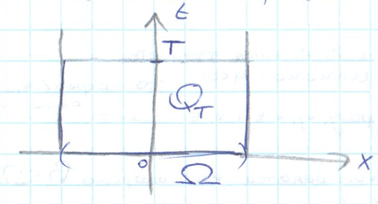
\includegraphics[scale=0.5]{part3.1.png}
\end{center}
% TODO: изображение

\begin{theorem}[Принцип максимума в ограниченной области]

Пусть $u$ --- классическое решение уравнения теплопроводности в ограниченной области $\Omega$. Тогда оно достигает максимума на $S_T$ для любого $T$.
\end{theorem}
\begin{proof}
Прежде всего стоит заметить, что максимум достигается, ведь $\overline{Q}_T$ --- компакт.

Обозначим точку максимума $u$ через $(t_0, x_0)$. Введем обозначение для оператора теплопроводности:
$$ Lu  = u_t - a^2 \Delta u.$$
Рассмотрим 
$$ v_{\eps} (t,x) = u(t,x) + \eps \abs{x}^2 \quad (\abs{v_{\eps}} > \abs{u})$$
Тогда
$$ L v_{\eps} = \pder[v_{\eps}]{t} - a^2 \Delta v_{\eps} = u_t - a^2 \Delta u - \eps a^2 \underbrace{\Delta \abs{x}^2}_{=2n} = Lu - 2 \eps a^2 n = - 2 \eps a^2 n.$$
Пусть $(t_{\eps}, x_{\eps}) \in \overline{Q}_T$ --- точка максимума $v_{\eps}$. Где именно она находится? Возможны три случая:

\begin{enumerate}
\item $(t_{\eps}, x_{\eps}) \in Q_T$ --- внутри цилиндра. Так как точка максимума находится в открытом множестве, то в ней все первые производные равны нулю, нас интересует $$v_{\eps, t} = 0.$$
В то же время в точке максимума вторые производные неположительны: $$ v_{\eps, x_i x_i} \leq 0, \quad \forall i \in 1:n $$
Получаем:
$$Lv_{\eps}  = \underbrace {v_{\eps,t}}_{=0} - \underbrace {a^2 \Delta v_{\eps}}_{\leq 0} \geq 0, \quad L v_{\eps} = -2n \eps a^2 < 0$$
Противоречие. Значит, $(t_{\eps}, x_{\eps}) \notin Q_T$.
\item $(t_{\eps}, x_{\eps}) \in \left\{ T \right\} \times \Omega$ --- на верхней крышке. По той же причине вторые производные по пространственным координатам неположительны:
$$ v_{\eps, x_i x_i} \leq 0.$$
Максимум достигается на правой границе временного интервала, значит,
$$v_{\eps,t} \geq 0$$
Имеем:
$$Lv_{\eps}  = \underbrace {v_{\eps,t}}_{\geq 0} - \underbrace {a^2 \Delta v_{\eps}}_{\leq 0} \geq 0, \quad L v_{\eps} = -2n \eps a^2 < 0$$
Противоречие. Значит, $(t_{\eps}, x_{\eps}) \notin \left\{ T \right\} \times \Omega$.
\item $(t_{\eps}, v_{\eps}) \in S_T$ --- на параболической границе. Единственный оставшийся вариант.
\end{enumerate}
Имеем:
$$ u(t,x) \leq v_{\eps} (t,x) \leq \max_{S_T} v_{\eps} \leq \max_{S_T} u + \eps \underbrace {(\diam \Omega)^2}_{=\const} \xrightarrow[\eps \to 0]{} \max_{S_T} u.$$
Таким образом, максимум $u$ достигается на $S_T$.

\end{proof}

\begin{corollary}[Принцип минимума]
Пусть $u$ --- классическое решение уравнения теплопроводности в ограниченной области $\Omega$. Тогда оно достигает минимума на $S_T$ для любого $T$.
\end{corollary}
\begin{proof}
Аналогично, только вместо $u$ рассматриваем $-u$.

\end{proof}

\begin{corollary}[Единственность]
Начально-краевая задача в $\Omega$
\begin{gather*}
	\begin{cases*}
		u_t - a^2 \Delta u = f, \\
		u \Big\rvert_{\partial \Omega} = h, \\
		u(0, x) = g.
	\end{cases*}
\end{gather*}
может иметь не более одного решения.
\end{corollary}
\begin {proof}
Пусть $u_1$ и $u_2$ --- решения. Тогда их разность удовлетворяет соответствующему однородному уравнению:
\begin{gather*}
	\begin{cases*}
		L(u_1 - u_2) = 0, \\
		(u_1 - u_2) \Big\rvert_{\partial \Omega} = 0, \\
		(u_1 - u_2) \Big\rvert_{t = 0} = 0.
	\end{cases*}
\end{gather*}
Из однородного уравнения разность наших решений равна нулю на всей границе, а по доказанной теореме максимум и минимум разности достигаются на параболической границе $S_T \subset \real^+ \times \Omega$. Значит,
$$0 = \min (u_1 - u_2) \leq (u_1 - u_2) \leq \max (u_1 - u_2) = 0 \quad \Rightarrow \quad u_1 - u_2 \equiv 0$$

\end{proof}
\begin{corollary}[Поведение решений при $t \to \infty$] Рассмотрим температурное поле в ограниченной области $\Omega$:
\begin{gather*}
	\begin{cases*}
		u_t - a^2 \Delta u = 0, \\
		u \Big\rvert_{\partial \Omega} = 0, \\
		u \Big\rvert_{t = 0} = g.
	\end{cases*}
\end{gather*}
То есть, на стенках поддерживается нулевая температура, в начальное время задано температурное поле $g$, источников и стоков теплоты внутри области нет. Тогда
$$ u(t,x) \xrightarrow[t \to \infty]{} 0$$
равномерно по $x$ и экспоненциально по $t$.
\end{corollary}
\begin{proof}
Будем считать, что $0 \in \Omega$. Рассмотрим
$$ v(t,x) = A e^{-bt} \prod \limits_{i=1}^n \cos C x_i. $$
Так как $\Omega$ --- область ограниченная, то она лежит в некотором $n$-мерном кубе. Значит, можно подобрать $C$ так, чтобы каждый из косинусов был положителен. Выбор $C$ зависит только от диаметра $\Omega$. Далее, применим оператор теплопроводности к $v$:
$$ Lv = -b \cdot v(t,x) + n a^2 C^2 \cdot v(t,x) = (na^2C^2 - b) \cdot v.$$
Если $b = n a^2 C^2$, то $Lv = 0$. По этой формуле можем подобрать $b$. Теперь выбираем большое $A$ такое, что
$$ v(0,x) = A \prod \limits_{i=1}^n \cos C x_i > \max_{x \in \Omega} |g(x)|.$$

Имеем $$Lv = 0,\quad v(0,x) \geq \abs{g(x)},\quad v \geq 0 .$$ Рассмотрим
$$ w_{\pm} = v \pm u.$$
Тогда:
\begin{gather*}
	Lw_{\pm} = 0, \\
	w_{\pm}\Big\rvert_{\partial \Omega} = v\Big\rvert_{\partial \Omega} \pm u\Big\rvert_{\partial \Omega} \geq 0, \\
	w_{\pm}\Big\rvert_{t=0} = \underbrace {v\Big\rvert_{t=0}}_{\geq \abs{g}} \pm \underbrace{u\Big\rvert_{t=0}}_{=g} \geq 0.
\end{gather*}

Таким образом, $w_{\pm}$ --- решения в $\real^n \times \Omega$ и положительны на $S_T$, а по принципу минимума $w_{\pm} > 0$  на $\real^n \times \Omega$. Из определения $w_{\pm}$ 
$$\abs{u(t,x)} \leq v(t,x) = A e^{-bt} \prod \limits_{i=1}^n \cos c x_i \xrightarrow[t \to \infty]{} 0.$$
Выбор констант $A$, $C$ и $b$ зависит только от $\diam \Omega$. Оценивая косинусы единицей, получаем, что
$$ \abs{u(t,x)} \leq A e^{-bt} \xrightarrow[t \to \infty]{} 0$$
равномерно по $x$, экспоненциально по $t$.

\end{proof}


\begin{note} Пусть существует классическое решение $\overline{u}$ задачи
\begin{gather*}
	\begin{cases*}
		\Delta \overline{u} = 0, \\
		\overline{u}\Big\rvert_{\partial \Omega} = h(x).
	\end{cases*}
\end{gather*}
Тогда для решения $u$ задачи 
\begin{gather*}
	\begin{cases*}
		u_t - a^2 \Delta u = 0, \\
		u \Big\rvert_{\partial \Omega} = h(x), \\
		u(0, x) = g(x)
	\end{cases*}
\end{gather*}
верно, что $$u \xrightarrow[t \to \infty]{} \overline{u}$$
равномерно по $x$, экспоненциально по $t$.
\end{note}

\begin{proof}
Рассмотрим $v = u - \overline{u}$. Тогда
\begin{align*}
& Lv = Lu - L\overline{u} = 0, \\
& v\Big\rvert_{\partial \Omega} = h - h = 0, \\
& v\Big\rvert_{t = 0} = g(x) - \overline{u}(x).
\end{align*}
Заметим, что $v$ удовлетворяет условию следствия. Значит, $ v \xrightarrow[t \to \infty]{} 0$, и $ u \xrightarrow[t \to \infty]{} \overline{u}$ равномерно по $x$, экспоненциально по $t$.

\end{proof}